\section{Theoretical Background}

\subsection{Big Data}
The term \textit{Big Data} roughly describes the enormous datasets that have become the norm in many industries over the past two decades. A 2014 report found, for example, that Facebook produced log data of over 10 \ac{pb} per month. \cite[]{chen_big_2014}

- increasingly relevant if current trends continue \cite[]{fan_mining_2013}

- existentially relevant for technology companies wanting to be future-proof

\subsection{Artificial Intelligence}
\ac{ai}, the field of research that occupies itself with giving machines the ability to think and learn, has been the focus of much research in recent years due to the increasing capabilities of hardware to tackle the challenges it involves

\subsection{Machine Learning}
\ac{ml} is a subfield of \ac{ai} in which machines extract information and patterns from data without thorough or explicit instructions, usually making use of highly contrived data from which noise (irrelevant or distracting background information) has been removed. Classifying objects based on a finite set of input values (e.g. birds based on their weight, wingspan, the colour of their back and whether they have webbed feet \cite[]{harrington_machine_2012}) is an ideal task for machine learning.

\ac{ml} tasks are generally split into two categories: supervised and unsupervised learning \cite[]{kelleher_fundamentals_2015}. The former involves training the model to associate input data with known output data and using it on previously unseen data; in the latter, a model is given data and instructed to find patterns or groups based on input data alone \cite[]{goodfellow_deep_2016}.

\subsubsection{Polynomial Regression}

\subsection{Deep Learning}
\ac{dl} is an application of \ac{ml} that employs more complex models capable of making sense of noisier, largely unprocessed data, such as sound signals and images \cite[]{goodfellow_deep_2016}. Classifying birds could in this case involve extracting necessary information from an image or diagram of the bird, requiring far less manual measurement or input.

\ac{dl} has seen a huge rise in popularity in recent years, with applications including speech recognition \cite[]{deng_machine_2013}, medical diagnoses \cite[]{lee_diagnosis_2018}, stock market prediction \cite[]{krollner_financial_2010} and many others \cite[]{kelleher_fundamentals_2015}. One particular challenge among the \ac{dl} research community is time series data \cite[]{yang_10_2006}, a sequential collection of values recorded over time. Time series data remains a great challenge due to its noisy, multidimensional nature \cite[]{kelleher_fundamentals_2015} and the dfficulties involved in developing algorithms that can also interpret the temporal information held in the signal \cite[]{bagnall_great_2017}.

\subsubsection{Multilayer Perceptron}
- diagram

- weight, bias, output, optimisation
\cite[]{kirk_thoughtful_2017}

- The quintessential DL network: Multilayer perceptron

\subsubsection{Time Series Classification}
\ac{tsc} involves reading time series data and applying one of a finite number of labels to each instance \cite{fawaz_inceptiontime_2019}.

The UCR Archive \cite{dau_ucr_2019} is a large collection of datasets released to enable research and offer a benchmark dataset to evaluate newly proposed \ac{dl} approaches.

The greatest breakthroughs in \ac{tsc} have only come about within the past few years since the publication of the Inception module \cite[]{szegedy_going_2014} and its subsequent application in further DL fields \cite{ismail_fawaz_deep_2019, fawaz_inceptiontime_2019}.

- OK for binary damage classifications, but in its original form (i.e. from \cite[]{fawaz_inceptiontime_2019}) the classes are not ordinal.

\subsubsection{Time Series Regression}
- Changing activation function of final TSC layer to linear and loss function to MSE as with the initial MLP, we can perform a regression on input

- Expect promising results with large datasets but to be taken with a pinch of salt: we now have infinite/continuous inputs AND outputs, therefore probably unscalable!

\subsection{The Engine}
The Civil Aerospace department of Rolls-Royce designs and manufactures primarily high-bypass turbofan jet engines, which offer an ideal arrangement for civil aircraft flying below the speed of sound \cite[]{rolls-royce_plc_jet_2015}.

Engines consist of four main components (fan, compressor, combustion chamber and turbine) which correspond approximately to the four stages of a Brayton cycle (intake, compression, combustion, expansion). The engine draws in air, compresses it, burns fuel in the compressed air and forces this air out through the rear nozzle, while extracting some energy at the turbine stage to continue powering the fan and compressor \cite[]{rolls-royce_plc_jet_2015}.

Many modern civil aircraft engines are equipped with two concentric shafts, split into \ac{lp} and \ac{hp}, which connect respective sets of compressors and turbines \cite[]{spittle_gas_2003}. Some, including the Rolls-Royce Trent family of engines, also have a third shaft, coupling the \ac{ip} compressor and turbine. Figure \ref{fig:triple_spool} shows the configuration of such an engine.

\begin{figure}
    \centering
    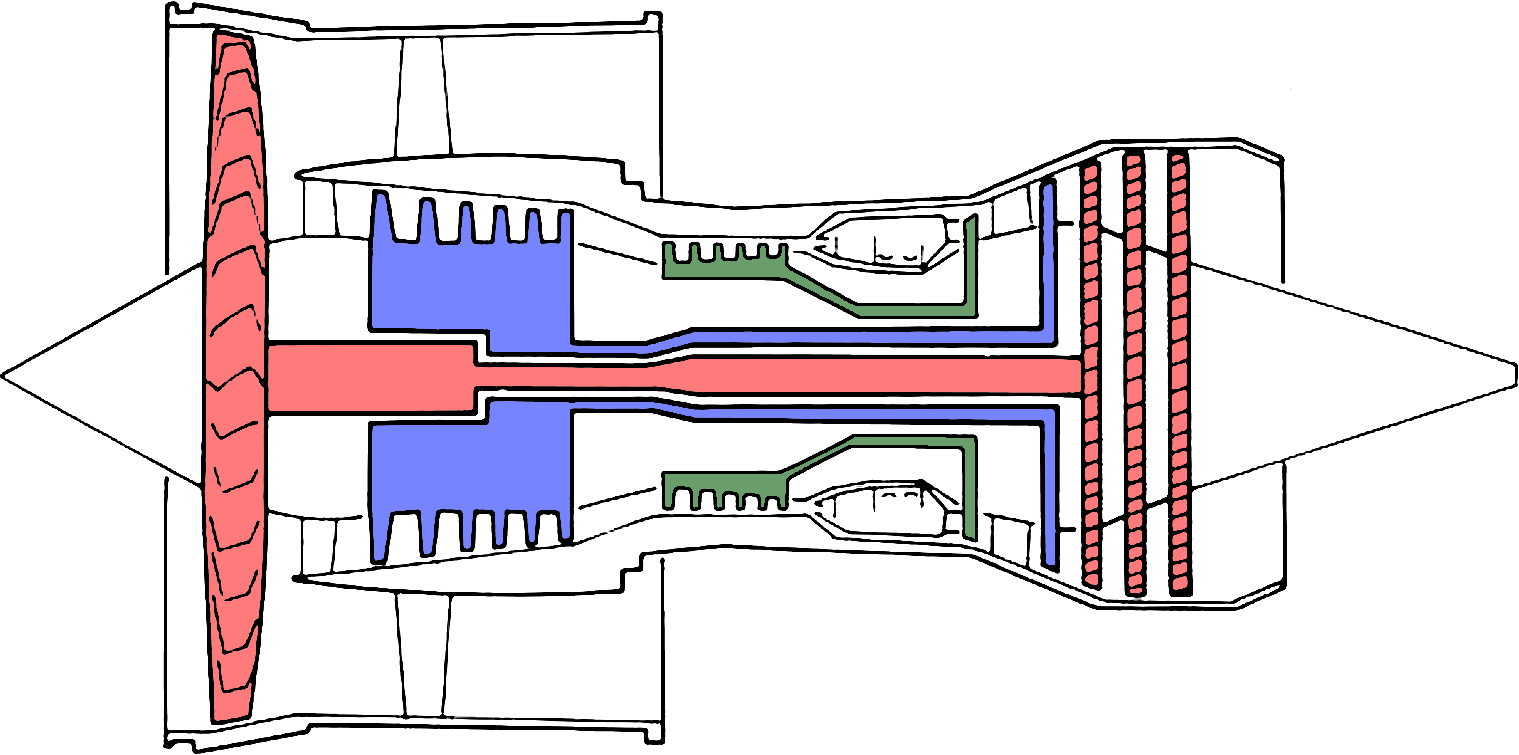
\includegraphics[width=0.7\textwidth]{triple_spool}
    \caption{\label{fig:triple_spool} A schematic diagram of a triple-spool high-bypass engine with \ac{lp}, \ac{ip} and \ac{hp} components shown in red, blue and green, respectively (based on \protect\cite[]{rolls-royce_plc_jet_2015}).}
\end{figure}

This multi-spool arrangement allows higher temperatures, pressures and rotational speeds in the engine, and thereby enables a higher pressure ratio with lower specific fuel consumption \cite[p. ~20]{rolls-royce_plc_jet_2015}. Despite these much improved thermal and propulsive efficiencies \cite[p. ~225]{rolls-royce_plc_jet_2015}, the arrangement comes with the compromise of significantly increased thermal and mechanical loads within the engine, particularly as the air passes from the combustion chamber to the \ac{hpt}. The \ac{tet} has risen to such an extent that \ac{hpt} blades now operate in temperatures far above their melting point, requiring great improvements in the materials, structures and systems used, such as extracting cooler air from the compressor stage and releasing this through air holes in the blades to create an insulating barrier between the blade and hot air \cite[]{spittle_gas_2003}.

\subsection{Damage}
Components used in such extreme conditions experience degradation. They therefore cannot be used indefinitely and must be removed from service after a certain amount of time to avoid potentially catastrophic failure. The amount of time for which the component is permitted for service, referred to as its Approved Life, is determined in safety analyses \cite[]{easa_certification_2015}. Approved Life is measured in Engine Flight Cycles, to be referred to as \textit{cycles} in the following. (These aspects will be discussed in more detail in Section \ref{certif}.)

The degradation of the engine through its use is referred to as damage. The extent of damage is dependent on many parameters: Since operators use their aircraft for different purposes, flight parameters such as duration, altitude and outside temperature vary greatly and result in different levels of damage. This idea can be quantified with the aforementioned cycles.

In a \ac{fe} context, components are modelled digitally and separated into a finite number of individual elements, the corner points of which are called nodes. Areas of particular interest within the component (usually where stresses are expected to be highest) are referred to as features.

Within Rolls-Royce, damage from flight missions is currently calculated using one of two internal tools for flight profile analysis: SA66 and Perseus (see Sections \ref{sa66} and \ref{pers}, respectively). The former is ideal for processing many flights in a short amount of time, but is restricted to a low number of features due to the time involved in manually setting up the surrogate \ac{fe} model for each feature. The latter can be described as a brute-force method that determines damage for all surface nodes, but is restricted by the amount of time required to process a single flight.

\subsubsection{Certification}
\label{certif}
Certification of a new engine includes a thorough safety analysis as described in \cite{easa_certification_2015}.

Of primary concern for the Rotatives department is the \ac{hpt} disk due to the extreme conditions under which it operates and therefore the risk of Hazardous Engine Effects. The latter is defined to include (among others) \textquote{non-containment of high-energy debris}, \textquote{uncontrolled fire}, \textquote{complete inability to shut the engine down} according to the \ac{easa} and the \ac{faa} \cite{easa_certification_2015, faa_guidance_2007}. A safety analysis must show that Hazardous Engine Effects are expected to occur with a probability no greater than \(10^{-7}\) per flight hour.

Engine parts whose failure is likely to result in Hazardous Engine Effects are labelled Engine Critical Parts \cite{easa_certification_2015}; the \ac{hpt} disk also carries this label. Engine Critical Parts are assigned an Approved Life, which defines the \textquote{mandatory replacement life} \cite{easa_certification_2015} of the part and is measured in Engine Flight Cycles, a flight profile that defines a reference flight mission, corresponding approximately to the average flight for which the engine is expected to be used in service.

Determining a part's Approved Life, commonly referred to as lifing, is a complex process, the majority of which involves \textquote{defining the duty the part is required to sustain} \cite{corran_lifing_2007}, i.e. the design and refinement of the Engine Flight Cycle. One lifing philosophy is that of \ac{ltfc}, which involves determining the \ac{pscl} by means of statistically-determined safety factors.

\subsubsection{SA66 Cycle Counter}
\label{sa66}
surrogate FE model

\subsubsection{Perseus}
\label{pers}


\subsection{Research Question}
Using the methods described in this section, the research goal of this thesis is to identify a supervised \ac{ml} or \ac{dl} approach that offers a sufficiently robust, verifiable, comprehensive, scalable, fast and accurate means of processing \ac{ehm} data to determine the extent of damage incurred by surface nodes of a component during real flight missions.